\onecolumn
\appendix
\section{Appendix}
\label{appendix}

Table and Figure numbers continue from the main document.  In the appendix are:
\begin{enumerate*}
  \item examples of game summaries written by  players (Table~\ref{tab:userfeedback});
  
  \item the game engine view of the board (Figure~\ref{fig:board});
  
  \item examples of persuasion techniques (Table~\ref{tab:persuasion});
  
  \item \wordlist{} word lists that are used as features in the logistic regression model (Table~\ref{tab:wordfeatures}); and

 \item A full transcript between two players, \player{Germany} and
\player{Italy} (Table~\ref{tab:transcript}).  Messages are long and carefully composed. This transcript is from the game described in Section~\ref{sec:walkthrough} (Warning: it is twenty pages long).
\end{enumerate*}



\begin{table}[h!]
	\centering
	\begin{tabular}{p{1cm} p{13cm} }
		\bf User & \bf                     Summary \\
		\toprule
		\noalign{\vskip 2mm} 
		Italy &This was an interesting game, with some quality play all around, but I felt like I was playing harder than most of the others. I felt early on that I could count on Austria remaining loyal, which worked to my benefit, as it allowed me freedom to stab and defeat a very strong French player before he got his legs under him. At the same time, Austria was a little too generous in granting me centers and inviting me to come help him against Russia, which allowed me to take advantage once I was established in the Middle Atlantic. \\
		\hline
		\noalign{\vskip 2mm} 
		Russia &Definitely a good game by Italy - which is interesting to me, because his initial press struck me as erratic and aggressive, making me not want to work with him. I'm curious if the same negotiating approach was taken with the other players who did work with him early on, or if he used a different negotiating approach with closer neighbors.\\
		\bottomrule
	\end{tabular}
	\caption{Users optionally provide free response descriptions of the game.  This can be used for qualitative analysis or potentially for algorithmic summarization.}
	\label{tab:userfeedback}
\end{table}


\begin{figure*}[b!]
	\centering
	\includegraphics[width=.8\linewidth]{\figfile{map_v2.pdf}}
	\caption{The board game as implemented by Backstabbr.  Players place moves on the board and the interface is scraped.}
	\label{fig:board}
\end{figure*}


%\begin{table*}[]
%	\centering
%	\footnotesize
%	\begin{tabular}{ l c c c c }
%		
%		&\multicolumn{2}{c}{\textbf{\alie{}}} & \multicolumn{2}{c}{\textbf{\slie{}}} \\
%		\toprule
%		\textbf{}            & \textbf{Lie \fone{}}     & \textbf{Macro \fone{}} & \textbf{Lie \fone{}}   & \textbf{Macro \fone{}}       \\ 
%		\hline			
%		\textbf{Baselines} \\
%		\midrule
%		Random     & 0.189  & 0.419 & 0.174  & 0.401	\\ 
%		Predict all as  Lie  &  0.214  & 0.107	& 0.186  & 0.093 \\ 
%		Predict all as Truth & 0.000   & 0.468   & 0.000  & 0.473  \\ 
%		Human      & 0.243 & \textbf{0.574}	& N/A & N/A\\ 
%		%\textbf{Logistic Regression}      &      0.72*                   &                        \\ 
%		\midrule
%		\textbf{Logistic Regression}\\
%		\midrule
%		%Game Features  & 0.00 & 0.00 & 0.00 & 0.00 \\
%		Language Features & 0.235  & 0.483  & 0.135 & 0.358 \\
%		Bag of Words & 0.184 & 0.525  &  0.142 & 0.516 \\
%		\midrule
%		\textbf{Neural} \\
%		\midrule
%		%Word &  0.03     & 0.49	  & 0.03    & 0.50	 \\ 
%		LSTM & 0.192    & 0.551	   &  0.138 & 0.531	 \\ 
%		LSTM + BERT & 0.216 &  0.559 & 0.203 & 0.542 \\
%		LSTM + Context  & 0.263 & 0.555 & 0.174   &  0.532 \\
%		LSTM + BERT + Power & 0.224 & 0.564 & 0.230 & 0.530 \\
%		LSTM + Context + Power & \textbf{0.287 }& 0.565  & 0.208 & \textbf{0.552} \\
%		LSTM + BERT + Context + Power & 0.257 & \textbf{0.571}  & 0.156 & 0.534 \\
%		\bottomrule
%	\end{tabular}
%	\caption{Test set results for both our \alie{} and \slie{} tasks.  The neural model that integrates past messages and power dynamics approaches human performance. }
%	\label{tab:results}
%\end{table*}

\begin{table*}[t]
	\centering
	\begin{tabular}{p{2cm} p{12cm} }
	\bf Principle & \bf    Example \\
	\toprule
	\noalign{\vskip 2mm} 
	Authority  & Sent to Germany, England, Austria, Russia: So, England, Germany, Russia, y'all played a great turn last turn. You got me to stab my long-time ally and you ended our pretty excellent 7-year run as an alliance. Russia told me he was with me if I stab Austria. England told me he wanted me to solo so long as I would ``teach him'' and help his along to second place. Then y'all pulled the rug out from under me. It was clever and effective. 
	At this stage, my excitement about the game has diminished quite a bit. And of course I'm happy to play on and take my lumps for falling for ``Hey, I really want you to solo, just help me place second,'' but if you guys just want to call it a five-way draw among us and grab a beer together, while reviewing the statistics, that's really my preference. 
	
	I am outnumbered and I obviously can't solo. And I'm sure some of you in the north are eager to send everyone else flying my way, but I expect Russia and England to be careful, and so I'm not sure there is much room to move forward without simply tipping the board to Germany's favor. 
	
	I propose that we draw and hug it out.\\
	\hline
	Reciprocity  & 1) You've been straight with me all game. 2) You have a much better ability to read the board than she does. 3) You're on the other side, so you can't really stab me, but I could totally see her moving to Tyrolia some time soon. 4) You're not in France's pocket. \\
	\hline
	Likability & Maine is beautiful! I used to go to scout camp there. \\
	\hline
	Scarcity & I'd like to have your final thoughts on A/R as quickly as possible so that I have time to execute a plan. But I understand if you want time to think about it.\\
	\bottomrule
	\end{tabular}
\caption{Examples of persuasion from the games annotated with tactics from \citet{cialdini2004social}.}
\label{tab:persuasion}
\end{table*}


\clearpage

\begin{longtable}{p{2 cm}  p{12cm} }
	\bf Feature & \bf Key Word \\
	\endfirsthead
	\toprule
	claim  & accordingly, as a result, consequently, conclude that, clearly, demonstrates that, entails, follows that, hence, however, implies, in fact, in my opinion, in short, in conclusion, indicates that, it follows that, it is highly probable that, it is my contention, it should be clear that, I believe, I mean, I think, must be that, on the contrary, points to the conclusions, proves that, shows that, so, suggests that, the most obvious explanation', "the point I'm trying to make", 'therefore, thus, the truth of the matter, to sum up, we may deduce\\
	\hline
	subjectivity  & abandoned, abandonment, abandon, abase, abasement, abash, abate, abdicate, aberration, aberration, abhor, abhor, abhorred, abhorrence, abhorrent, abhorrently, abhors, abhors, abidance, abidance, abide, abject, abjectly, abjure, abilities, ability, able, abnormal, abolish, abominable, abominably, abominate, abomination, above, above-average, abound, abrade, abrasive, abrupt, abscond, absence, absentee, absent-minded, absolve, absolute, absolutely, absorbed, absurd, absurdity, absurdly, absurdness, abundant, abundance, abuse, abuse, abuse, abuses, abuses, abusive, abysmal, abysmally, abyss, accede, accentuate, accept, acceptance, acceptable, accessible, accidental, acclaim, acclaim, acclaimed, acclamation, accolade, accolades, accommodative, accomplish, accomplishment, accomplishments, accord, accordance, accordantly, accost, accountable, accurate, accurately, accursed, accusation, accusation, accusations, accusations, accuse, accuses, accusing, accusingly, acerbate, acerbic, acerbically, ache, achievable, achieve, achievement, achievements, acknowledge, acknowledgement, acquit, acrid, acridly, acridness, acrimonious, acrimoniously, acrimony, active, activist, activist, actual, actuality, actually, acumen, adamant, adamantly, adaptable, adaptability, adaptive, addict, addiction, adept, adeptly, adequate, adherence, adherent, adhesion, admirable, admirer, admirable, admirably, admiration, admire, admiring, admiringly, admission, admission, admit, admittedly, admonish, admonisher, admonishingly, admonishment, admonition' \dots \\
	\hline
	expansion  & additionally, also, alternatively, although, as an alternative, as if, as though, as well, besides, either or, else, except, finally, for example, for instance, further, furthermore, however, in addition, in fact, in other words, in particular, in short, in sum, in the end, in turn, indeed, instead, later, lest, likewise, meantime, meanwhile, moreover, much as, neither nor, next, nonetheless, nor, on the other hand, otherwise, overall, plus, rather, separately, similarly, specifically, then, ultimately, unless, until, when, while, yet\\
	\hline
	contingency  & accordingly, as a result, as long as, because, consequently, hence, if and when, if then, in the end, in turn, indeed, insofar as, lest, now that, once, since, so that, then, thereby, therefore, thus, unless, until, when\\
	\hline
	premise  & after all, assuming that, as, as indicated by, as shown, besides, because, deduced, derived from, due to, firstly, follows from, for, for example, for instance, for one thing, for the reason that, furthermore, given that, in addition, in light of, in that, in view of, in view of the fact that, indicated by, is supported by, may be inferred, moreover, owing to, researchers found that, secondly, this can be seen from since, since the evidence is, what's more, whereas\\
	\hline
	temporal-future & after, afterward, as soon as, by then, finally, in the end, later, next, once, then, thereafter, till, ultimately, until\\
	\hline
	temporal-other  & also, as long as, before, before and after, earlier, in turn, meantime, meanwhile, now that, previously, simultaneously, since, still, when, when and if, while\\
	\hline
	comparisons & after, although, as if, as though, besides, by comparison, by contrast, conversely, earlier, however, in contrast, in fact, in the end, indeed, instead, meanwhile, much as, neither nor, nevertheless, nonetheless, nor, on the contrary, on the one hand on the other hand, on the other hand, previously, rather, regardless, still, then, though, when, whereas, while, yet\\
	\bottomrule
	\caption{The word lists used for our \wordlist{}~\cite{niculaelinguistic} logistic regression models.} \label{tab:wordfeatures}
\end{longtable}
\clearpage
\twocolumn


\clearpage
\onecolumn
\dpcomment{update with Truth/Lie instead of True/False }
\begin{longtable}{p{.3 cm} p{1.25cm} p{8.25cm} p{1.1cm} p{1.1cm}}
		\label{tab:transcript}
		\bf \# & \bf Speaker & \bf  Message  & \bf Actual Lie & \bf Suspected Lie \\
		\toprule
		\endfirsthead
		%\noalign{\vskip 2mm} 
		0 & Italy & Germany!
		
		Just the person I want to speak with. I have a somewhat crazy idea that I've always wanted to try with I/G, but I've never actually convinced the other guy to try it. And, what's worse, it might make you suspicious of me. 
		
		So...do I suggest it?
		
		I'm thinking that this is a low stakes game, not a tournament or anything, and an interesting and unusual move set might make it more fun? That's my hope anyway.
		
		What is your appetite like for unusual and crazy? & Truth & Truth \\
		\hline
		1 & Germany & You've whet my appetite, Italy. What's the suggestion? & Truth & Truth \\
		\hline
		2 & Italy & Okay, don't hate me!  Key West (Just thought of the name lol)
		
		Basic point is that I move to Tyr in Spring and into Mun in the Fall, while I take Tun with my fleet. I build A Ven/F Nap. 
		You open to Ruh/Hol/Kie, and force Belgium. 
		You wind up with 2 builds, and the sympathy and concern of your neighbors who are astonished at the crazy Italian. ``What a stupid move, he can't hold Munich!''
		Trap is set to obliterate France in the Spring of 02. Bel S Mun - Bur, Ven - Pie, Tun - WMed. 
		France won't see it coming, He will see that attack on Munich and think that both you and I will be occupied for a while. So Spring 02 should be a serious surprise. 
		
		Now, you're taking risk here, because you're giving up a home center for a turn hence the ``Key''), but I think you can see pretty clearly that I derive no benefit from trying to double-cross you. After all, Italy trying to hold Munich is just dumb. I'm from a school of thought that even trying to move to Munich is just dumb. But this would be the one exception. I can't hold Munich, and even if I wanted to, it would give me an awkward snake formation in the middle of the board that is a great way to be first eliminated.  So I think this works because you know (even more than Austria in a traditional Key Lepanto), that I'm not going to stab you. And doing it this way allows us to take Burgundy by surprise, it ensures you get Belgium, and it crushes your biggest rival and toughest border (France). 
		Plus, it'll be fun. 
		The Key West! 
		Thoughts?   \textit{*This message crashed the Beta version of the bot due to its length and is not in the dataset.  It is manually extracted and added here the purposes of readability*}
		& Truth & None \\
		\hline
		3 & Germany & It seems like there are a lot of ways that could go wrong...I don't see why France would see you approaching/taking Munich--while I do nothing about it--and not immediately feel skittish & Truth & Truth \\
		\hline
		4 & Italy & Yeah, I can't say I've tried it and it works, cause I've never tried it or seen it. But how I think it would work is (a) my Spring move looks like an attack on Austria, so it would not be surprising if you did not cover Munich. Then (b) you build two armies, which looks like we're really at war and you're going to eject me. Then we launch the attack in Spring. So there is really no part of this that would raise alarm bells with France.
		
		All that said, I've literally never done it before, and it does involve risk for you, so I'm not offended or concerned if it's just not for you. I'm happy to play more conventionally too. Up to you. & Truth & None \\
		\hline
		5 & Italy & I am just sensing that you don't like this idea, so shall we talk about something else? That was just a crazy idea I've always wanted to try. I'm happy to play more conservatively. & Truth & None \\
		\hline
		6 & Italy & Any thoughts? & Truth & None \\
		\hline
		7 & Germany & Sorry Italy I've been away doing, um, German things. Brewing Lagers? & Truth & Truth \\
		\hline
		8 & Germany & I don't think I'm ready to go for that idea, however I'd be down for some good ol'-fashioned Austria-kicking? & Truth & Lie \\
		\hline
		9 & Italy & I am pretty conflicted about whether to guess that you were telling the truth or lying about the ``brewing lagers'' thing. I am going to take it literally and say thumbs down even though I don't think you meant it deceptively.  & Truth & Truth \\
		\hline
		10 & Italy & But I think I can get over ``Lagergate'' and we can still be friends. 
		
		As of right now, I think Austria may be my most reliable ally. I'm thinking I'd like to play as a Central Trio if you have any interest in that. Thoughts? & Truth & Truth \\
		\hline
		11 & Germany & We haven't even passed a season yet and you have a 'most reliable ally'?
		
		I'll consider this proposal but, basically, I'm not going to expose myself to risk from either of you until I've seen a bit of your behavior & Truth & Truth \\
		\hline
		12 & Italy & Well, at least I have an idea of who to trust. Obviously, my ideas are subject to change. 
		
		I understand your desire to watch behavior before committing to anything. I, personally, am a partner player. I look carefully early in the game for a small group to work with, and then I value loyalty and collaboration. I like to work closely with a tight-knit alliance. 
		
		If you prefer to hop and back and forth, or play more of an individual game, then we might not be a good match. 
		
		I'm looking for a loyal ally or two that I can coordinate with and make awesome moves with. Makes the game easier and a lot more fun. & Truth & Truth \\
		\hline
		13 & Italy & Just an FYI: I've now had both England and France suggest to me that I should move to Tyrolia and France will support me to Munich in the Fall. One saying that to me is not a big deal, but with both mentioning it, my alarm bells are going off. I am concerned about an E/F. 
		
		I'm certainly not moving to Tyrolia. But I just want you to be cautious here. I feel like England and France are working together. & Truth & Truth \\
		\hline
		14 & Germany & I appreciate the tip, but I'm wondering why you're so against ousting me from Munich if I haven't explicitly agreed to be your ally? & Truth & Truth \\
		\hline
		15 & Italy & Because it is terrible, terrible play for Italy to attack Germany, in my view. If I were to attack you in Munich, I could never hold Munich. So, all I would be doing is weakening you, and helping France, England, or both to get really big. 
		
		I don't have any long-term path going north. Helping France to take you down is a sucker's play, whether you are working with me or not. & Truth & None \\
		\hline
		16 & Italy & Did France tell you he was moving to Burgundy, or was that a stab? & Truth & Truth \\
		\hline
		17 & Germany & I was not informed of it, no. And England is leading me to believe it's part of a play for Belgium, so if they're working together this might be a trick...
		
		Italy, you seem like a straight shooter, and Austria has confirmed with me about your two's alliance. So I'll confide in you--this is my first ever game of diplomacy, and I think that teaming up with the two of you could help me learn more and have more fun. So, if you're still interested in a central powers alliance, I'm in. & Truth & Truth \\
		\hline
		18 & Germany & Okay full disclosure: I'm not very smart, and I accidentally let slip to England that you told me France was plotting to take Munich. I'm sorry for the error but I figured it was better to admit it so you know that England/France may not trust you. & Truth & Truth \\
		\hline
		19 & Italy & Okay, thanks for telling me. & Truth & Truth \\
		\hline
		20 & Germany & So, um, no alliance then? & Truth & Truth \\
		\hline
		21 & Italy & I do want to be allies. Sorry, busy weekend here running around with bambinos. More to come. & Truth & Truth \\
		\hline
		22 & Germany & What would you think of helping me take Marseilles in two turns? & Truth & Truth \\
		\hline
		23 & Italy & Hi Germany, I'll certainly consider that. Though, I'll note: traditionally, Germany would help Italy to Marseilles if the two of them work together there. The reason is that: if I help you to Marseilles, I'm basically cut off from going west and getting anything myself. So, usually, Germany would help Italy into Marseilles to encourage Italy to come west and Germany would plan to take Paris, Belgium and Brest. & Truth & Truth \\
		\hline
		24 & Germany & Fair enough--I'll help you take it, then, but I'll need to deal with Belgium first. & Truth & Truth \\
		\hline
		25 & Italy & How are things going with England? I think that getting him to work with you is the main key here. & Truth & Truth \\
		\hline
		26 & Germany & I'm trying--I just offered to assist with taking Sweden in exchange for some assistance into Belgium...not sure if they'll go for it... & Truth & Truth \\
		\hline
		27 & Italy & I'll check with England and try to see where his head is at. & Truth & Truth \\
		\hline
		28 & Germany & I've actually been thinking about this game all day  and have come up with a plan I like a bit better... but England still hasn't responded to my initial offer. & Truth & None \\
		\hline
		29 & Italy & That's the worst!
		
		And I'm glad to see you're so focused on this in your first game. It's a really great game if you put in the time and effort! & Truth & Truth \\
		\hline
		30 & Germany & You're definitely telling the truth on that one. So can I count on you to move to piedmont this season? & Truth & Truth \\
		\hline
		31 & Italy & I don't think I can afford to move to Piedmont this season. I don't really trust Austria to avoid walking through that door if I leave it wide open. 
		
		I think you need to get England on board to attack France. & Truth & Truth \\
		\hline
		32 & Germany & That's valid. And actually I was conferring with England and we concluded that it's not really gonna be possible for me to help you take Marseilles this year anyway. 
		
		...what are you and Austria planning for this year, then? I'm willing to tell you my plans in exchange as a gesture of trust. 
		
		Have you communicated at all with England or France? & Truth & Truth \\
		\hline
		33 & Italy & Hi, are you there?
		
		Just woke up. 
		
		England did return my message, but he did not tell me anything substantive so I really don't know what he's doing. I'm planning to move towards Turkey. & Truth & Truth \\
		\hline
		34 & Italy & Well, you're in trouble. That England move is trouble. 
		
		I'm going to try to convince him to change course. I suggest you be very kind to him, and don't burn that bridge. I think your game hinges on turning England around. & Truth & Truth \\
		\hline
		35 & Italy & Hi Germany,
		
		I'm working hard on turning England. And I'm also trying to get Russia to come to your aid. Doing the best I can! I'll keep you posted. & Truth & Truth \\
		\hline
		36 & Germany & England just told me that Russia is helping them to take Denmark so that may be a lost cause. Granted, the source for that intel is a serpentine jackal-spawn & Truth & Truth \\
		\hline
		37 & Italy & Okay, I'm reasonably sure that England wants to take the Channel and attack France now. 
		
		I believe that you should basically do whatever England asks to help make this happen. As long as E attacks F, you will be in a much better position, and you'll gain back centers quickly. 
		
		What are you hearing? & Truth & Truth \\
		\hline
		38 & Germany & What are your plans for this turn? I can't help but notice that Munich is surrounded by foreign armies on three sides...
		
		I wish I could be more helpful but I'm pretty much just treading water right now trying not to lose anything else & Truth & Truth \\
		\hline
		39 & Italy & Hey --- sorry, just getting back into this now. & Truth & Truth \\
		\hline
		40 & Italy & I have good news! (1) I am finally attacking France this turn. (2) I will be supporting Munich to hold from Tyrolia. 
		
		Let's turn this game around, yes? & Truth & Truth \\
		\hline
		41 & Italy & I am pretty sure that England is not attacking you this turn. And I am committed to supporting Munich holding. Make sure you don't move Munich so that it can take my support. & Truth & Truth \\
		\hline
		42 & Germany & Okay, can do. Thanks! & Truth & Truth \\
		\hline
		43 & Italy & I suggest that you order:
		Kiel Support Berlin holding
		Berlin Support Munich holding
		Helg to Holland
		Munich Support Berlin holding & Truth & Truth \\
		\hline
		44 & Germany & I agree completely--although I didn't know that a country could hold *and* support at the same time! Thanks! & Truth & Truth \\
		\hline
		45 & Germany & Thanks Italy. Hope you're enjoying the weather on the Anatolian & Truth & Truth \\
		\hline
		46 & Italy & I will be supporting Munich to hold again. And I'll be trying to get Russia to back off your flank and protect himself against an Austrian stab that is coming. & Truth & None \\
		\hline
		47 & Italy & Two bits of advice: \#1 I suggest you tell Russia that Austria is coming for him. You really want Russia to move Sil back to Gal. You might also suggest to Russia that is he supports you to Denmark, you will then support Russia back to Sweden. I don't know yet if it actually makes sense to do that, but you want Russia thinking that you are eager to work with him. He'll be hoping for a reason to break off his attack on you at this point. & Truth & None \\
		\hline
		48 & Italy & \#2 Here is the move set I would suggest right now:
		Kiel Support Holland holding
		Holland Support Wales to Belgium (tell England you are going to order this support and he can take it or leave it)
		Munich Support Berlin holding
		Berlin Support Munich holding
		
		I think that both France and Russia are about to back off you, as they are both under fire at home. Just hold still, and soon you should be able to break out of this holding pattern. & Truth & None \\
		\hline
		49 & Germany & God, I hope so! I'm attempting to make that deal with russia now...and I'm talking with England re: Belgium & Truth & Truth \\
		\hline
		50 & Italy & It's none of my business, but if you do plan to take Denmark, I strongly recommend you wait until Fall. I think the most important thing for you right now is getting England fully committed against France. If that happens, taking Denmark later will be easy. & Truth & Truth \\
		\hline
		51 & Germany & I think me and England are really on the same page at this point regarding France. I'm actually sort of running counter-intelligence for England (and my friends to the south, of course!) with Russia right now. 
		
		England and I talked about Denmark too...and it seems like one or the other of Denmark or Belgium should work out for me this year and I'm fine with that & Truth & Truth \\
		\hline
		52 & Italy & Great to hear. Thank you. & Truth & Truth \\
		\hline
		53 & Germany & Do you need me to disrupt Bur this year? I'll need to seriously trust Russia if I'm going to risk not holding my eastern front, I think... & Truth & Truth \\
		\hline
		54 & Italy & I do think a move to Burgundy makes sense for you this turn, and I can't imagine Russia attacking you here. He has a serious Austria problem. 
		
		I suggest this:
		Mun - Bur
		Ruh - Bel
		Hol Support Ruh - Bel 
		Ber - Kie
		
		Tell Russia that the last thing in the world you want to see is Austria run him over, and you're willing to help keep Russia viable if necessary (you're angling for Russia to disband his northern holdings this turn). & Truth & Truth \\
		\hline
		55 & Italy & And ask England nicely to support Ruh - Hol, with the explanation that you don't plan to ask for Denmark back, but you think it would help you both to diminish France. (You'll get Den back eventually, but you want England to think you don't care about it). & Truth & Truth \\
		\hline
		56 & Germany & Thanks, I'll work on these. 
		...Why didn't you scooch into the Aegean behind Austria? You could have defended or even held Bulgaria this turn? & Truth & Truth \\
		\hline
		57 & Germany & England and I were talking about your moves for this season--what do you think of convoying Pie into Spa, supporting this with Wes, and then moving Tyr into Pie? & Truth & Truth \\
		\hline
		58 & Germany & This leaves Marseilles open for Bur to fall into if France goes that route, which gives me an opening into Bur & Truth & Truth \\
		\hline
		59 & Italy & That's not bad. & Truth & Truth \\
		\hline
		60 & Italy & I was kind of thinking I should pick one or the other of Marseilles or Spain to attack and not tell a soul which one I'm going after. & Truth & Truth \\
		\hline
		61 & Italy & Do you really think it's important to coordinate? & Truth & Truth \\
		\hline
		62 & Italy & I do think you're best off moving to Burgundy. And there is some chance that we fail this turn. But I think we just take a guess and hope for the best. We'll get him next turn if not this one. & Truth & Truth \\
		\hline
		63 & Germany & Okay---sorry for being nosy! I will try for bur on the off chance it shakes out that way & Truth & Truth \\
		\hline
		64 & Italy & Nah, you're not being nosy at all. I mean, come on, we both know that I have no problem sticking my nose where it doesn't belong. & Truth & Truth \\
		\hline
		65 & Germany & Marked as true & Truth & Truth \\
		\hline
		66 & Italy & I like to coordinate, but on these sort of 50/50 guesses, I kind of like to keep it secret so that if it doesn't go well, I have nobody to blame but myself. & Truth & Truth \\
		\hline
		67 & Italy & Ha! & Truth & Truth \\
		\hline
		68 & Germany & Well, are you willing to humor my question about the Aegean, anyway? & Truth & Truth \\
		\hline
		69 & Italy & Sure. I was thinking of moving that fleet to Ionian. You think a move to Aegean is better? I'm not really sure, but let's talk it through. & Truth & Truth \\
		\hline
		70 & Germany & No sorry I meant in hindsight--like this past turn you should have moved to Aeg so that this current turn, when Austria takes Rumania (from Bulgaria), you'd be there to cover Bulgaria so it couldn't get scooped by the Black sea, and potentially you'd just get to take it. & Truth & Truth \\
		\hline
		71 & Italy & Not a bad point. I agree. & Truth & Truth \\
		\hline
		72 & Italy & Hmmmm, kind of a pointless lie if you ask me, but I won't hold it against you. You're in a tough spot. & Truth & Truth \\
		\hline
		73 & Germany & um what lie? I did exactly the moves you suggested! & Truth & Truth \\
		\hline
		74 & Italy & Ha! So sorry!! I meant that for France! & Truth & Truth \\
		\hline
		75 & Italy & You are my favorite. & Truth & Lie \\
		\hline
		76 & Germany & Marked as lie because clearly austria is your favorite.
		Speaking of, I assume that your seizing Trieste was mutually agreed upon? & Truth & Truth \\
		\hline
		77 & Italy & Yes --- agreed upon. & Truth & Truth \\
		\hline
		78 & Germany & That's not what Austria said to England... & Truth & Truth \\
		\hline
		79 & Italy & Hmmmm, okay. Well, let's just keep that between you and me then. & Truth & Truth \\
		\hline
		80 & Germany & You know Italy, I think we *do* need to coordinate your move this time--England and I have a shot at either Bur or Mao if one of Marseilles or Spain can be left open for France to fall into. This will improve all of our chances of crushing France quickly. & Truth & Truth \\
		\hline
		81 & Italy & Okay, I can dig it. What do you want me to do? & Truth & Truth \\
		\hline
		82 & Germany & Let me confer with England and get back to you. Glad to hear that though! & Truth & Truth \\
		\hline
		83 & Italy & So...any thoughts on how to approach this? & Truth & Truth \\
		\hline
		84 & Germany & It looks like England's not willing to try for MAO if it means possibly losing the channel. However, they'll bring the NWG fleet around to try for MAO next year. 
		So if you could keep Marseilles open, it will help me to try and take Burgundy this turn. & Truth & Truth \\
		\hline
		85 & Italy & If I leave Marseilles open, would you kindly use Burgundy in the Fall to help me take Marseilles? (Likely that means ordering Burgundy to Gascony to cut support) & Truth & Truth \\
		\hline
		86 & Germany & Will do. & Truth & Truth \\
		\hline
		87 & Germany & Okay, so I still have a teensy little bone to pick with you: on the off-chance that Austria wasn't lying and you *did* take Trieste unexpectedly, I sort of worry that I might be next. Are you willing to tell me what your plans are for the Tri unit, or at least to warn me before any move into Tyrolia? & Truth & Truth \\
		\hline
		88 & Italy & Sure. But, you'll see from my moves this turn that Austria is lying to you. & Truth & Truth \\
		\hline
		89 & Italy & I currently have Tri - Tyrolia. I like the unit there because it sets up an attack on Austria if I ever want to go that route (build A Ven and go east). Do you want me to keep Tyrolia clear? & Truth & Truth \\
		\hline
		90 & Italy & I'll add --- I would never attack Germany as Italy. Setting myself as a giant column like that is just not defensible. It would be a terrible move. & Truth & Truth \\
		\hline
		91 & Germany & Not when that column is not-so-giant and in a turf war with France. & Truth & Truth \\
		\hline
		92 & Germany & oh you mean setting *yourself* & Truth & Truth \\
		\hline
		93 & Germany & But you could easily pick off, say, Munich and not be a "giant column" & Truth & Truth \\
		\hline
		94 & Italy & I mean this sincerely: any Germany who does that is a terrible player. 
		
		Why would I do that? I would need 2-3 units to hold one center. That is a net negative. And all of your units are doing things that are good for me in containing your neighbors. 
		
		I've been working hard in this game for you to succeed and knock back France and England. I can say with 100\% certainty: I'm not going to attack you. I'm going to keep helping you as much as I can. & Truth & Truth \\
		\hline
		95 & Italy & That said, if you want me NOT to move to Tyrolia, I won't move there. & Truth & Truth \\
		\hline
		96 & Germany & Nah, I just needed some reassurance :)
		Your logic is undenyable--- enjoy your stay in tyr! & Truth & Truth \\
		\hline
		97 & Germany & *undeniable? That looks better & Truth & Truth \\
		\hline
		98 & Italy & I mean it sincerely. I think that England will want to coax me to attack you with him after France falls, but I'd much rather work with you against England. 
		
		But first thing's first --- let's get rid of France. & Truth & Truth \\
		\hline
		99 & Germany & Agreed & Truth & Truth \\
		\hline
		100 & Germany & (On the france part) & Truth & Truth \\
		\hline
		101 & Germany & Sorry I won't be able to cut off Gascony this turn...I probably should have just told you my moves; you could have advised me that supporting Mun-Bur was more important than Kie-Ruh & Truth & Truth \\
		\hline
		102 & Italy & No worries. We'll crack this but eventually. 
		
		Here is my suggestion for this turn:
		Kie - Den
		Hol S Bel holding
		Bel S Ruh - Bur
		Mun S Ruh - Bur
		Ruh - Bur & Truth & Truth \\
		\hline
		103 & Italy & I think you should suggest to England that he gets Sweden and St Petersburg, while you get Denmark back. That's only fair, as you have been a loyal ally in the fight against France and you plan to continue to do that. & Truth & Truth \\
		\hline
		104 & Germany & The moves I had already planned differ in one respect: I thought it would be worth the risk to try moving Hol-Bel and therefore move Bel-Bur. Even if me and France are high-fiving in Bel for a few seasons it's still mine, and it's not like Holland has anything better to do while I'm still allies with England.
		
		...The only reason I'm reluctant to make that agreement with England is that---while I think *you* and I have a good relationship---I really have not talked with Austria much at all, and I'm the next logical target for them when Russia's gone. And anything that's bad for Russia right now is good for Austria. & Truth & Truth \\
		\hline
		105 & Italy & Hmmmm, I'm just not sure you should trust England enough right now to leave Holland open and Belgium essentially unguarded. 
		
		France is a really good player, and he is no doubt working hard to get England to turn on you. My personal take is that you are better off being a bit more conservative until you have Denmark back and England has moved another fleet towards France. But I can see it either way. & Truth & Truth \\
		\hline
		106 & Italy & With regard to Russia, talk it through with England. What you don't want is England taking out Russia and giving you nothing. So, if England agrees to let Russia be for a while, then your plan sounds good. But if England is going to take Sweden, you really should get Denmark back. (I'm my view) & Truth & Truth \\
		\hline
		107 & Germany & Okay you've convinced me: it's worth figuring out what E's plans are for Russia at least.
		
		And you're almost certainly right, from a rational perspective, about leaving Holland/Belgium vulnerable to England. But I think England really is counting on my assistance in taking France, and because of that and other non-quantifiable reasons I trust them. & Truth & Truth \\
		\hline
		108 & Italy & Excellent. Obviously you have a much better feel for your relationship with England than I do. Just know that France is persuasive, and I'm sure that's what he's working on. He stopped talking to me, so I bet he's trying to turn England. Just keep reassuring England that you want to work with him long-term so he doesn't succumb to the Dark Side. & Truth & Truth \\
		\hline
		109 & Italy & Hi Germany --- well, I think we're getting to a critical point in the game here. France held out a long time, but he's much less of a threat now. I think the critical issue, for you, is England. 
		
		I have some thoughts on the matter, and some information, but I'd like to feel confident that you and I will keep anything we say between us. I think of you as the one person who has been honest with me on every turn. You even tell me the truth when it's bad news, or when you don't completely trust me, and I like that. & Truth & Truth \\
		\hline
		110 & Germany & Okay, Italy. I won't share any of this conversation. But in the interest of continued full disclosure, here's what I think: England is a greater threat to *me* on the map, but *you* have a greater chance of soloing this game quickly, or pair-winning with Austria even sooner. And if I continue to collaborate with England, we at least have a chance of slowing that down. So I'm in sort of a conflicted spot & Truth & Truth \\
		\hline
		111 & Italy & This is why I like you. The full disclosure part. You tell me the truth even when the news isn't great. & Truth & Truth \\
		\hline
		112 & Italy & My thoughts on the ``Germany/England forever so that at least we can stop the solo'' strategy: (1) It's quite early to be talking about solos. I am at 8, and Austria could take 3 from me any time, quite easily. (2) I don't think England is thinking that way. I think he's thinking that a dominant power will emerge in the north, and one will emerge in the south. And he's like to be that dominant power. & Truth & Truth \\
		\hline
		113 & Italy & England's pieces are not positioned well if he's trying to attack France or contain Italy. He keeps Denmark guarded, and North Sea filled. He is not playing like he intends to stick with you, even though I'm sure he's telling you that. & Truth & Truth \\
		\hline
		114 & Italy & You're right that you don't want to start a war with England right now. But, you must stick up for yourself, because nobody else will do that if you don't. & Truth & Truth \\
		\hline
		115 & Italy & If I were you, this is what I would do: (1) keep warning England about the dangers of Italy getting too big and insist that England moves his fleets towards MAO (Channel to Irish, Norwegian to NAO, North - Channel), (2) insist on taking Denmark back. & Truth & Truth \\
		\hline
		116 & Italy & I would say something like this:
		
		England, I'm with you my friend, but we're passed the stage of you needing to keep me under lock and key. I need to take Denmark back. I'm happy to support you to Brest to keep you growing, or you can grab Sweden. You have plenty of options other than keeping your ally's center, but if you really want to be my ally long-term, you've got to show me that. & Truth & Truth \\
		\hline
		117 & Italy & I am hearing from England signs that he may be thinking of attacking you soon. And I think you actually avoid that better by being strong and sticking up for yourself rather than being accommodating and letting him do whatever he wants to do. & Truth & Truth \\
		\hline
		118 & Germany & Well, both you and France have now pointed out that England is strategically not in a good place to be my ally right now, and you are correct. I'll be more cautious with my northern border, but I made a pretty strong argument for denmark this past turn and it fell on deaf ears & Truth & Truth \\
		\hline
		119 & Germany & ...which probably also should have been a sign for me & Truth & Truth \\
		\hline
		120 & Italy & Well, if you want, you could just take Denmark this next year and I don't think England is in a position to retaliate. & Truth & Truth \\
		\hline
		121 & Germany & Probably not...has France been talking with you at all about their sunsetting strategy? They've indicated a willingness to work with you and me and a desire to see England get as few dots as possible & Truth & Truth \\
		\hline
		122 & Italy & He did say that to me too. Though, France has a long history of lying to me, so I really don't trust him. & Truth & Truth \\
		\hline
		123 & Germany & Well France has actually been pretty honest with me, and I at least am certain that they wouldn't betray me to England. So, I'm considering working with F to sabotage (or potentially full-on backstab) England this turn, which would have the side-effect of maybe taking some attention away from the south for you anyway. & Truth & Truth \\
		\hline
		124 & Germany & (and I'd be interested to hear your thoughts on this if you're in the mood to give out free advice) & Truth & Truth \\
		\hline
		125 & Italy & Hi Germany --- sorry for the delay. Well...I think it's really important that you get a build this turn either way. I don't think England will get a build this turn, so if I were you I'd probably take Paris, build a fleet, and move on England after that. & Truth & Truth \\
		\hline
		126 & Italy & But it likely depends on how communication is going with England. If he'll give you back Denmark, that might change the equation. & Truth & Truth \\
		\hline
		127 & Germany & I am waiting on England to make a decision about that--they claim to be thinking about it. & Truth & Truth \\
		\hline
		128 & Germany & England told me you said I was plotting with France. It makes sense you'd want to pit us against each other. & Truth & Truth \\
		\hline
		129 & Italy & Hey --- tried to send you a message earlier but not was down. England was telling me that you're saying that I told you that England is plotting against you. The problem with telling England that is that he will stop giving me useful info. & Truth & Truth \\
		\hline
		130 & Italy & Truly, I don't want you and England to fight. I am not trying to break you up. I suggested that you take Paris! I want you guys to work together with me against France. & Truth & Truth \\
		\hline
		131 & Germany & You don't want us to fight, yet you betrayed both of our confidence with you in a way that makes us distrust each other? & Truth & Truth \\
		\hline
		132 & Italy & I really don't think that's a fair description. You guys both wanted to attack each other. I encouraged you both to keep working together. & Lie & Truth \\
		\hline
		133 & Germany & Just as long as it suits you. Are you going to give England Mao? & Truth & Truth \\
		\hline
		134 & Italy & Hmmm, should I be reading that as angry sarcastic with dagger eyes? (I'm not sure if I'm getting your tone right) & Truth & Truth \\
		\hline
		135 & Italy & We're friends, right? I believe that every single message I've sent you all game has been truth, and I've gone out of my way to give you candid advice. Are we still friends? & Lie & Truth \\
		\hline
		136 & Italy & Regarding MAO --- I don't know. What do you want me to do? I don't have any set plan. & Truth & Truth \\
		\hline
		137 & Germany & Yep, there's some sarcasm there. Looking back at your messages, I still don't read them as encouraging collaboration. And if you wanted us to be friends, you could have done that without betraying me to England by simply saying in your candid way "I don't think you should do that for such and such reason". But you chose to increase E's distrust of me. So I think you might be full of gnocchi and crap. 
		
		My trust in you is a bit shaken but I still think we can have a working partnership with a bit more caution on my end. It would be my preference that you hold Mao, on the assumption that if it came down to a choice between partnering with me or England, you'd choose me. If that's not the case, then as the filling of an England-Italy sandwich I'm in no position to retaliate anyway. & Truth & Truth \\
		\hline
		138 & Italy & Well, again, I like that you're honest with me, even when the news is bad. & Truth & Truth \\
		\hline
		139 & Italy & I have to say that I'm surprised that you feel that I've betrayed your trust. I have been feeling like maybe I've been TOO helpful to you, and been a bit over the top in offering advice, etc., but it seems like I've misread the situation. & Lie & Truth \\
		\hline
		140 & Germany & No, it's completely true that you've been too helpful, and I'm really really grateful for it because I've been able to learn so much from this game. But it's also true that you didn't have to tell England what you did, and all you stood to gain from it was that it shook my and E's trust in each other. & Truth & Truth \\
		\hline
		141 & Italy & But I understand what you're saying, and I much prefer to have a heart to heart like this, a frank airing of grievances, rather than being surprised by unkind moves on the board. https://youtu.be/xoirV6BbjOg & Truth & Truth \\
		\hline
		142 & Germany & Was not expecting seinfeld today and it was a pleasant surprise & Truth & Truth \\
		\hline
		143 & Italy & :) & Truth & Truth \\
		\hline
		144 & Italy & Here's the deal: I like you better than England. & Lie & Truth \\
		\hline
		145 & Italy & I'm not sure how the next couple of turns are going to shake out. But I like that you tell me when you're angry with me. I know that may seem like a small thing, but it's just rare in Diplomacy. You get so many fake smiles. & Truth & Truth \\
		\hline
		146 & Italy & So, if it comes down to you or him, I'm choosing you. And I'll work to do a better job of keeping your confidence. I certainly understand how important that is, as I hate it when people o that same thing to me. & Truth & Truth \\
		\hline
		147 & Italy & So no more playing mediator for me. & Truth & Truth \\
		\hline
		148 & Germany & Okay. Is it true that you want the channel? & Truth & Truth \\
		\hline
		149 & Germany & And are you planning to keep Vienna? & Truth & Truth \\
		\hline
		150 & Italy & I am not planning to keep Vienna. And yeah I've asked France for support to the Channel. Do you think he's on board? & Truth & Truth \\
		\hline
		151 & Germany & I'm not sure. Is *England* on board? Is this something England can know about? & Truth & None \\
		\hline
		152 & Italy & No, do you think France will Support me to the Channel? & Truth & Truth \\
		\hline
		153 & Germany & France has asked my opinion on it, and I haven't given it yet. To my estimation things look a lot better for me if you don't end up there: I don't want to see England in Mao, and I don't want to see you snagging pieces of the north. & Truth & Truth \\
		\hline
		154 & Italy & Okay, well, here is my thinking. Tell France whatever you want to make him happy. Then tell me how you really feel. And if you don't want me to go there, I won't go there. & Truth & Truth \\
		\hline
		155 & Germany & If I hadn't asked you about it, would that have just been another surprise, too? & Truth & Truth \\
		\hline
		156 & Italy & Absolutely. 
		
		You and I have discussed our moves and been honest with each other every turn. But we have not been sharing all our moves or pre-clearing all of our moves. So that would have Ben a surprise in the same way that your moves are a surprise to me. (I never tell you what to do or insist on knowing). & Truth & Truth \\
		\hline
		157 & Italy & I kind of thought that you would have wanted me in the Channel because it commits me further against England, but I can understand what you're saying now about wanting me to hang back. & Truth & Truth \\
		\hline
		158 & Italy & But I don't think there is anything wrong with me contemplating moves without telling you all of them. You asked me about it, and I told you the truth. & Lie & Truth \\
		\hline
		159 & Germany & I do think that this move is a breach of general expectation, which is the kind of thing I'd like to know about. And it's also the kind of thing I've shared with you: case in point, my desire to stab England. & Truth & Truth \\
		\hline
		160 & Italy & Okay. Understood. & Truth & Truth \\
		\hline
		161 & Germany & Is there anything I could gain from seeing you in the channel? Would you support me taking Nth, and potentially seizing the island? & Truth & Truth \\
		\hline
		162 & Germany & Here's what I'm thinking: I would be on board with you taking the channel (and I'd give France the green light to go ahead with it) if you would agree to bump Nao out of Mao using Wes, and if you'd be open to supporting some anti-English aggression while holding the channel so that I can get on equal footing with you, dot-wise.
		
		If you don't want to agree to those terms, that's okay, but I would strongly prefer not to see you in the channel in that case. & Truth & Truth \\
		\hline
		163 & Italy & I'm going to be out of pocket this weekend, so let's talk this through more on Monday. Generally, I agree that I'll either stay out of the Channel or agree to your terms for entering there. & Truth & Truth \\
		\hline
		164 & Germany & If you decide to stay out of the channel, I have a deal that I like with England in the works. For that deal to go through, you'd have to agree to move Mao into Portugal to let England take Mao. Would you be amenable to that? & Truth & Truth \\
		\hline
		165 & Germany & (If this second offer is more to think about than a no-brainer, you can just mull it over and let me know monday) & Truth & Truth \\
		\hline
		166 & Italy & So, here is my concern with the England offer: If I'm taking Portugal, why do we want England in MAO? And why would he want to go to MAO? I'm not sure I understand that one. Can you explain? & Truth & Truth \\
		\hline
		167 & Germany & Well, when I initially proposed the deal I had forgotten that Portugal was promised to England. Then England agreed to it on the condition that you would confirm that move, so I figured E thought you would just move out of there next year? But now that I think about it, it's probably worth asking England why they'd agree to that. & Truth & Truth \\
		\hline
		168 & Italy & I'd prefer that you not tell England I am considering moving to the Channel. I don't think he would like that. & Truth & Truth \\
		\hline
		169 & Italy & I don't really want to discuss this stuff with England at all. & Truth & Truth \\
		\hline
		170 & Germany & Well, England changed their mind about the plan I offered anyway. So, are you taking the channel? & Truth & Truth \\
		\hline
		171 & Italy & No, I'm not taking the Channel. & Truth & Truth \\
		\hline
		172 & Germany & Okay was that a recent decision? Because like an hour ago France said they were supporting you into the channel & Truth & Truth \\
		\hline
		173 & Italy & Well, when I tell you what I plan to do, do you turn around and tell France? This makes me uncomfortable speaking with you. & Truth & Truth \\
		\hline
		174 & Germany & I haven't spoken to France since then. I didn't realize you were giving the two of us different information on this particular subject. But I don't think I've revealed anything to them about what you plan to do. Mostly because you haven't told me. & Truth & Truth \\
		\hline
		175 & Italy & Well, I have been honest with both you and France. You told me that I need to promise you a set of things in order to take the Channel. I felt like it was more than I could be sure of doing, so I am not entering the Channel. I won't go there without your permission. & Lie & Truth \\
		\hline
		176 & Germany & I appreciate that. And I'll keep the remainder of this conversation between us unless I hear otherwise. Have you just recently made an agreement with England? & Truth & Truth \\
		\hline
		177 & Germany & I heard as much but I want to verify the contents of that agreement with you & Truth & Truth \\
		\hline
		178 & Germany & Btw, France just said that they submitted the orders to support you into the channel. & Truth & Truth \\
		\hline
		179 & Italy & I don't have an agreement with England, but he is asking me about my moves and trying to get my help. & Truth & Truth \\
		\hline
		180 & Germany & Okay--then England is lying to me, saying that you're helping support Eng-Brest. & Truth & Truth \\
		\hline
		181 & Italy & Ha! Yeah, fat chance. & Lie & Truth \\
		\hline
		182 & Germany & ...but did you lie to England about that? Or can I say to England that I don't think you'll actually provide that support? & Truth & Truth \\
		\hline
		183 & Italy & What is Paris up to? & Truth & Truth \\
		\hline
		184 & Italy & I suggest you just not tell England anything about my moves. & Truth & Truth \\
		\hline
		185 & Italy & Do you want me to support England to Brest? & Truth & None \\
		\hline
		186 & Italy & I guess I'm not sure what your goals are here. & Truth & Truth \\
		\hline
		187 & Italy & I just kind of feel like you're grilling me with a lot of questions, but not telling me what you're doing or what you want from me. & Truth & Truth \\
		\hline
		188 & Germany & *If* you support Eng-Brest, England has agreed to vacate denmark for me. If you don't, I won't get in the way of your channel thing. Any other questions? & Truth & Truth \\
		\hline
		189 & Germany & I have no sense of what you want or what your plan is, but I thought I'd been pretty clear: I want Denmark. I am reluctant to see you in the Channel if England remains powerful, but happy to see you there if they are weakened. & Truth & Truth \\
		\hline
		190 & Italy & Can't you just force Denmark? & Truth & Truth \\
		\hline
		191 & Germany & Not without risking a swipe of Belgium & Truth & Truth \\
		\hline
		192 & Germany & And why force when you don't have to & Truth & None \\
		\hline
		193 & Italy & Okay, I'll support England to Brest. You take Denmark. & Truth & Truth \\
		\hline
		194 & Italy & And you and I should be in position to take out England next year. & Truth & Truth \\
		\hline
		195 & Germany & Splendid! & Truth & Truth \\
		\hline
		196 & Germany & Glad everything worked out & Truth & Truth \\
		\hline
		197 & Italy & Thumbs up! & Truth & Truth \\
		\hline
		198 & Italy & Congratulations on retaking Denmark and getting two builds. You are playing really well right now. Respect. & Truth & Truth \\
		\hline
		199 & Germany & Congrats on having double-digit dots! I have some thoughts about taking out England, if you want to go full-stab this season... & Truth & Truth \\
		\hline
		200 & Italy & I think I do! & Truth & Truth \\
		\hline
		201 & Italy & What are you thinking? & Truth & Truth \\
		\hline
		202 & Germany & One option is to take the channel, another is to take Brest. Between you, me, and Picardy we can manage either, but it's a question of which takes priority. If we chose Brest, I could also take a stab at seizing Nth this season, then we could try for the channel in fall. Or we could do channel first, Brest second. & Truth & Truth \\
		\hline
		203 & Italy & Yeah, that is all along the lines of what I'm thinking. How demanding does France sound right now? Does he want to be the one who takes Brest? & Truth & Truth \\
		\hline
		204 & Germany & Haven't asked. But in general not demanding. & Truth & Truth \\
		\hline
		205 & Italy & Good!
		
		Still, I think we should show him some good faith by supporting him to Brest in Spring. We can decide in Fall whether it makes more sense for you to take it, but I think we want to keep France hungry. & Lie & Truth \\
		\hline
		206 & Italy & I would suggest something like this to ensure the English fleet is disbanded:
		Pic - Bre
		MAO - Channel
		Par S Pic - Bre & Lie & Truth \\
		\hline
		207 & Italy & And Spa - Gas to cut off that retreat. & Truth & Truth \\
		\hline
		208 & Italy & You can take the North Sea on the same move and set up a convoy to the English mainland. 
		
		Checkmate. & Truth & Truth \\
		\hline
		209 & Germany & Okay, I like the plan! I've asked France if they're willing to move to Brest supported by me. & Truth & Truth \\
		\hline
		210 & Germany & Aren't you concerned about England taking Mao? I'd sooner just have you pile on support into Bre so that Wes can support Mao holding & Truth & Truth \\
		\hline
		211 & Italy & That's a good point, but the problem with that approach is that Brest is not guaranteed. If England cute MAO and supports with the Channel, the attack fails. I think we are better off ensuring that the Brest fleet is disbanded. If we disband that fleet and take North Sea, an English fleet in MAO really just spreads him out and allows you to take the island faster. It's not like he can get Portugal or Spain. & Truth & Truth \\
		\hline
		212 & Germany & Okay, but that means I'd prefer to take Brest myself this Spring, if France is okay with it. & Truth & Truth \\
		\hline
		213 & Italy & I think that we should offer France Brest in Spring. That ensures that he is with us. Then, if conditions are right in the Fall, I can support you into Brest. But...England can offer France Belgium, and I think he is sure to take that if we're not even offering him a center, right? & Lie & Truth \\
		\hline
		214 & Italy & Better to keep France feeling like we're going to keep him in the game. If you need the build in Fall, it's easy for me to support you there. & Lie & Truth \\
		\hline
		215 & Germany & I guess I'm just wondering from France's perspective why they'd *want* to stay in the game. Isn't it possible they'd rather move on with their life? That's not rhetorical, I'm wondering what your perspective is as a veteran player & Truth & Truth \\
		\hline
		216 & Italy & Here is my take: If France just wanted to go down in a blaze of glory and say ``eff you'' to England, he would have kept Irish Sea. He kept Pic, which is next to his home center, and gives him a chance to negotiate with both you and England. & Lie & Truth \\
		\hline
		217 & Italy & I think that means he is motivated to keep trying. And if he believes he can get Brest, he could legitimately get back to his feet. I know that's what I'd be trying to do in his position. & Truth & Truth \\
		\hline
		218 & Italy & As the poker saying goes: ``a chip and a chair.'' So long as you have one chip left, and you're still in the tournament, you can always come back to win. & Truth & Truth \\
		\hline
		219 & Italy & Thoughts? & Truth & Truth \\
		\hline
		220 & Germany & I think that makes sense. Are you talking with England at all? & Truth & Truth \\
		\hline
		221 & Italy & I'm pretty wary of England right now. He asked me what I want to do, but I feel like he's trying to get me to leave MAO open. That's not terrible news, as it suggests that he won't expect your move to North Sea. & Lie & Truth \\
		\hline
		222 & Italy & As long as he doesn't move NAO to Norwegian, you've got a guaranteed supply center. & Truth & Truth \\
		\hline
		223 & Germany & Well E'd have to be a right dolt not to retreat to NWG. And right now they're talking to me about supporting a move from Bre to Gas (the better for the two of us to stab you). & Truth & Truth \\
		\hline
		224 & Germany & What i mean is, there's a good chance that Mao is safe if I "agree" to that deal & Truth & Truth \\
		\hline
		225 & Germany & Oh nevermind--they're not going to convoy into Brest. So actually this pretty much guarantees that Eng and Nao will try for Mao. & Truth & Truth \\
		\hline
		226 & Italy & Ahhhh, sneaky Devil! Thank you for letting me know. & Lie & Truth \\
		\hline
		227 & Italy & I still like our plan. & Lie & Truth \\
		\hline
		228 & Italy & I need to run for a bit. I'll be around in a few hours. & Lie & Truth \\
		\hline
		229 & Germany & I think that knowing this, you should do as I suggest and not poke Eng. Just hold and let Wes support. I am 94\% sure I can trust England to do as they say on this one. & Truth & Truth \\
		\hline
		230 & Italy & Okay. Should I support Pic to Bre? & Lie & Truth \\
		\hline
		231 & Germany & yes please. It'll do us good with France too if we both support. & Truth & Truth \\
		\hline
		232 & Italy & Thumbs up! & Truth & Truth \\
		\hline
		233 & Germany & Actually, you should use Mao to support Spa-Gas, since we know that Brest is moving there. It will be beneficial to have you there if we decide to oust France from Bre in fall & Truth & Truth \\
		\hline
		234 & Italy & Consider it done. & Lie & Truth \\
		\hline
		235 & Italy & Hmmmm, heading anything from England? & Truth & Truth \\
		\hline
		236 & Italy & I'd love to talk if you're there. I'm getting the impression that England may actually be moving on you, and I think I have a good counter, but I also still think we should support the attack on Brest and take North Sea. & Lie & Truth \\
		\hline
		237 & Italy & I definitely think you should keep your moves the same. & Truth & Truth \\
		\hline
		238 & Italy & Nice! Get'em! He WAS moving on you. But we should be able to take about 3 off of him now. Very nice turn. & Lie & Truth \\
		\hline
		239 & Germany & Sorry; I was asleep by 9 last night  
		
		why the move to Nao? Wouldn't IRI be the more anti-England choice?
		
		With the move to Picardy and assuming a retreat to SKA, it looks like England has me pretty powerless this turn. & Truth & Truth \\
		\hline
		240 & Germany & So do you, it seems, if you have some kind of deal with Russia about Munich. & Truth & Truth \\
		\hline
		241 & Italy & Good morning. 
		
		Just responding to your messages above. I think NAO and Irish are equally anti-English. They both give me a clear lane to attack Liverpool. I wasn't sure if either one would be left open, but I took a gamble and it paid off. & Truth & Truth \\
		\hline
		242 & Italy & Re your move this turn, I don't think you're powerless. You should get a build I think and if not, you should be in position to smash England. & Lie & Truth \\
		\hline
		243 & Italy & I don't have a deal regarding Munich, Germany. Frankly, I thought you would be a bit more joyful towards me. By attacking England, I have committed completely to working as your partner. & Lie & Truth \\
		\hline
		244 & Germany & I suppose you're right. Initially I was thinking IRI also gives you channel access, but NWG access may be just as useful. 
		
		Well when you control half a continent (and even more when you consider your influence over me, austria, and who knows who else!), there's no such thing as complete commitment. I'm not so naive as to think your allegiance with me is going to last beyond its usefulness, and with two fleets on the British isle that time is fast approaching. To be clear, I'm still giving you the truth and I still want to work with you. But you should really stop acting surprised when I'm slightly paranoid that a soon-to-be-dozen-dot-holder is gearing up to stab me & Truth & Truth \\
		\hline
		245 & Italy & Well, I dunno, it sounds like I should stab you. Is that what you're trying to tell me?
		
		I like you. I like how hard you've worked in this game to rebound from a difficult start. I like that you e told me the truth, even when the news was bad. I like that you tell me when you don't trust me. I have literally never told you a lie in this game, and I don't intend to start now. Last turn I burned my bridge with England beyond repair. If you don't want to work with me now, that's really disappointing. & Lie & Truth \\
		\hline
		246 & Germany & like I said, I *do* want to work with you. However, remember that thing I said about general expectations and being warned when they're broken? Tyrolia is one of them and I think you knew that. And England *also* told me they've never told me a lie; I'm starting to think that's Diplomacy-speak for "when convenient, I've used careful wording and half-truths to deceive you even when everything I said was technically true". 
		
		It would help me to know that you see me being a benefit to you beyond taking out England. A natural next move for us would be to take out russia, and in that arena I have a positional advantage over you. Especially if I get two builds this turn, I'll be able to sneak behind the troops in bohemia/galicia and help you break through. & Truth & Truth \\
		\hline
		247 & Italy & Yes --- here is how I expect and hope the game will play out: the two of us finish off England and France, while drifting towards the east a bit. With the builds we get this year, we essentially blitzkrieg the East. I have more units than you, but you have no opposition at all in the north, and can take Scandinavia, War and Mos without any trouble. & Lie & Truth \\
		\hline
		248 & Italy & I think that, in about two years, you and I will both be on about 14 centers, with the remnants of Russia and Austria between us, and we can decide how we want to resolve it. I'd be happy to agree to a small draw, or to shoot for a 17-17 two-way draw position, whichever you prefer. & Lie & Truth \\
		\hline
		249 & Germany & Well, I like the sound of all of that. In fact, it sounds ideal: there's something poetic about the complete beginner and the expert (you've probably heard by now that you got doxxed) sharing a victory. 
		
		I ask for a concession: As a show of good will, would you be willing to take only one of Liverpool or Portugal this year? (I know the Portugal request seems weird, but I like keeping France around and unless I'm mistaken they like me better than you ) & Truth & Truth \\
		\hline
		250 & Italy & Yes. I wasn't planning to take Portugal anyway. & Truth & Truth \\
		\hline
		251 & Italy & I think it makes sense here for you to land an army in the English island while you can. Now that his army is off the island, he's toast as soon as you do that. & Lie & Truth \\
		\hline
		252 & Germany & England's just vindictive enough to try and stab Belgium with England and Picardy, though. I was planning on keeping holland around as support. & Truth & Truth \\
		\hline
		253 & Germany & *by England I of course mean Eng & Truth & Truth \\
		\hline
		254 & Italy & I suggest the following:
		
		Gas - Liv (via convoy)
		Spa S MAO holding
		Mar hold
		Tyr - Tri
		
		Hol - Yor (via convoy)
		Bur S Bel
		Bel S North
		HEL S North
		Mun - Boh
		Par - Pic (to cut any potential support) & Lie & Truth \\
		\hline
		255 & Italy & England cannot take Belgium with those moves. & Lie & Truth \\
		\hline
		256 & Italy & Or I could move my fleet into Liverpool and use Gas to support Bre. I'm happy either way. & Lie & Truth \\
		\hline
		257 & Germany & I tried a double convoy in the sandbox once and it didn't work! What is this witchcraft?!? & Truth & Truth \\
		\hline
		258 & Germany & At any rate, I prefer the fleet move to liverpool and Gascony's support into Brest. And could Mao support Bre into the Channel? No sense forcing France to disband. Bel will support it, too. & Truth & None \\
		\hline
		259 & Italy & Here are the orders needed to do a convoy!
		Holland move to Yorkshire
		North Sea convoy Holland to Yorkshire
		
		It is not a ``double convoy'' as you only need one fleet to make it happen. 
		
		But if your fleet in North Sea is dislodged, the convoy will not go through. That is why I would suggest that HELG supports North Sea holding and Belgium supports North Sea holding. & Lie & Truth \\
		\hline
		260 & Germany & No--I mean the one *you* were planning: Gascony to Liverpool & Truth & Truth \\
		\hline
		261 & Germany & It's a double convoy because you're convoying through Mao *and* Nao & Truth & Truth \\
		\hline
		262 & Italy & Ah, the orders there would be:
		Gascony - Liv
		MAO Convoy Gas - Liv
		NAO Convoy Gas - Liv & Truth & Truth \\
		\hline
		263 & Italy & So, I'll move the fleet to Liverpool. And you want MAO to support Paris to Brest? & Lie & Truth \\
		\hline
		264 & Italy & Or wait, MAO supports Brest to Channel, and Gas supports Paris - Brest, right? & Lie & Truth \\
		\hline
		265 & Germany & yeah. I tried that once in the sandbox (or the equivalent: back when you had fleets in Lyo and Wes I tried  a convoy from Pie to Naf). But I think I messed up the commands to the fleets. 
		
		And yes the most recent message is correct. Those two things and Nao-Lvp & Truth & Truth \\
		\hline
		266 & Italy & Okay, confirmed. 
		
		So I've got in:
		NAO - Liv
		MAO S Bre - Channel
		Gas S Par - Bre
		Spa - WES
		Mar S Gas holding 
		Tyrolia - Trieste
		
		Sound right? & Lie & Truth \\
		\hline
		267 & Germany & It does. But If Tyr was bound for trieste anyway, why did you detour through Tyr at all? Why not just move to trieste last turn?? & Truth & Truth \\
		\hline
		268 & Italy & Austria would not have liked it. & Truth & Truth \\
		\hline
		269 & Italy & And he doesn't know that it's headed back there now (please don't tell) & Truth & Truth \\
		\hline
		270 & Germany & Understood. Me and Austria don't talk anyway. Also, do you have any sense of what England is planning to do? & Truth & Truth \\
		\hline
		271 & Italy & Ha! No I don't. I'd imagine he is coming for me. But I don't know that. & Lie & Truth \\
		\hline
		272 & Italy & If I were him, I'd defend Edi and London. & Lie & Truth \\
		\hline
		273 & Germany & So you haven't been talking to England at all? I was sort of hoping you would know more, maybe help us take better advantage of their plans. & Truth & Truth \\
		\hline
		274 & Germany & Anyway, my moves are:
		
		Par-Bre
		Bel s Bre-Eng
		Hol s Bel holding
		
		And the rest within expected parameters. Correct? & Truth & Truth \\
		\hline
		275 & Italy & England has not said anything of substance to me. He was gracious about my move, but he won't trust me again, and I would not trust anything he might say at this point. I haven't asked him about his moves and he hasn't told me. & Lie & Truth \\
		\hline
		276 & Italy & I thought you would Convoy Holland to Yorkshire and support Belgium from Burgundy. Also, can you please order Mun to Boh to cut support and allow me to hold Vienna while moving Tyrolia to Trieste? & Truth & Truth \\
		\hline
		277 & Germany & I *told* you I'm not risking that convoy *and* that instead Bel is supporting France into the Channel (which will heretofore be called the French Channel). And could I persuade you to move to IRI instead of taking Liverpool in exchange for the requested cut? & Truth & Truth \\
		\hline
		278 & Italy & Sorry, what is the requested cut? I understand that you don't want me to take Liverpool or Portugal. What are you offering to me? (I don't mean to be difficult, I just want to be sure I understand). & Truth & Truth \\
		\hline
		279 & Italy & Ah, you must mean Munich to Boh. & Truth & Truth \\
		\hline
		280 & Italy & Asking me to avoid taking Por and Liv is asking a lot. I want France to survive here, but I also want England taking units off the board, and I feel like you should too, right? & Truth & Truth \\
		\hline
		281 & Germany & I do. But I also want those dots for myself, of course. And there's still the nonzero chance that you've arranged with Boh to take Munich for yourself, so I'm taking a serious risk & Truth & Truth \\
		\hline
		282 & Italy & I will avoid taking Portugal, vacate Tyrolia, and support you to Brest. I feel like I'm offering quite a lot in exchange for one cut support. 
		
		And cutting that support does not put you in greater peril. If I had a deal with Russia for Munich (I don't) I could cut Burgundy from Marseilles and support Russia to Munich. Moving Mun to Boh to cut support is costless. & Lie & Truth \\
		\hline
		283 & Germany & You're right. I just thought I'd put my best argument forward. I'll do the cut. But I ask for something costless in exchange, and I really, really want it to stay just between us, ok? & Truth & Truth \\
		\hline
		284 & Italy & Understood and agreed. & Truth & Truth \\
		\hline
		285 & Italy & And I have no problem with you asking for more than you're willing to settle for. That's smart, and I do the same thing sometimes. If you don't stick up for yourself, nobody else will. & Truth & Truth \\
		\hline
		286 & Germany & I *know* there's more to your relationship with England than you're telling me. The last message England sent to me hinted that if *I* wasn't willing to work with them--and I haven't said anything to them since--that maybe *you* would. And if England were to reach out to you, you're too smart to just snub them. There's advantage to be gained--either for both of us or just for yourself--from talking to them. The only reason I stopped was because I knew my word would be mud to them anyway.
		
		Earlier I was hoping you'd give me the truth about what you knew, and about what they might know. But you didn't and that both disappoints and scares me. So I'm asking that you give me just a modicum of honesty here: what do you know? what does England know? & Truth & Truth \\
		\hline
		287 & Italy & I give you my word: I don't know what England is going to do and I haven't asked. & Lie & Lie \\
		\hline
		288 & Italy & He is still jovial with me and respectful. He has asked me to critique his play and to give him advice. But I do not know his moves, and I really don't think he would tell me them if I asked. It certainly would not be info I could trust free I just lied to him about mine. & Lie & Truth \\
		\hline
		289 & Germany & But England's desperate. Better to talk with *someone* than just go in blind. And I doubt they'd turn to Russia or France because neither is really close enough/powerful enough to give real help. And there's precedent for you negotiating with someone even as you stab them: France.
		
		...and here's the real accusation: for all your pretty words about a shared victory between you and me, you've been sneaky and you've always pitted me and England against each other to your benefit. My real fear here is that knowing my moves, and with a desperate, jovial England seeking your advice, it would be so *easy* to just feed England enough info to keep me weak while you chow down on the Island. 
		
		I know this from experience: back when you were doing 50/50 shots in the south of France, I did everything I could to find out what you were planning and feed it to France. This was merely a time-buying measure, since France was outmatched and I would eventually run out of pretenses to extract your move. But I wanted to gain more dots before you took over. And I assume others are like me, hence I suspect you now. 
		
		I'm offering this confession in hopes that you'll do the same. So just come clean and let's approach this thing as equals? & Truth & Truth \\
		\hline
		290 & Italy & I am in my car, off to pick-up my kids from school. This deserves a proper response, so please give me some time. & Truth & Truth \\
		\hline
		291 & Germany & Abandon the children this is important & Truth & Truth \\
		\hline
		292 & Italy & So, I'm going to speak frankly here. I am rarely offended in a Diplomacy game, and I rarely say so when I am, but this message offends me. I'm trying to think about why I'm having such a strong reaction to it. I think it's because you're painting a picture of the game (both your actions and mine) which are totally different than my own perspective. (Continuing) & Lie & Truth \\
		\hline
		293 & Italy & From my perspective, you were on the ropes early. France and England were teaming up on you. You lost Denmark and France had Holland and Munich surrounded. You were in serious peril. 
		
		I seriously went to extreme effort to keep you in the game. I spent hours talking with England and encouraging him to turn around and go the other way. I completely ended my eastern campaign and spent two seasons just making the voyage over to France so that he didn't have the bandwidth to continue his attack. I have vouched for you with Austria and Russia many times. I have supported Munich. And I have NEVER attacked you, even when people have asked me to do so and pledged to support me. & Lie & Truth \\
		\hline
		294 & Italy & I have been honest with you, I have worked hard for your success, and I've made a lot of proposals to you in which you gain centers; not me. 
		
		Maybe I am just a bad ally, but I'm not sure I remember an alliance in which I have done more to help my ally. Truly. & Lie & Truth \\
		\hline
		295 & Italy & And to hear that (1) You think I've been selfish and (2) You've been sabotaging me all along, that just doesn't sit well with me. & Lie & Truth \\
		\hline
		296 & Italy & I have rarely asked for your help, and I've offered my help freely. I've provided my sincere best efforts to help you with tactics, and I have never sabotaged you. Not once. & Lie & Truth \\
		\hline
		297 & Italy & And if I'm totally honest with you, I could solo this game if I felt like lying to everyone and grabbing dots. I think I've got you all beat tactically. I just have more experience. But that's not been my intent. & Lie & Truth \\
		\hline
		298 & Italy & I've spent hours today talking with England about how best to play Diplomacy. I've tried to give him some honest advice because he asked for it. But I don't know his moves, I haven't asked for them, and I'm not going to take advantage of that relationship to try to stab you. It legitimately did not cross my mind until you accused me of doing it. & Lie & Truth \\
		\hline
		299 & Italy & So, I'm frustrated by this accusation. & Lie & Truth \\
		\hline
		300 & Germany & And I appreciate all you've done for me, really I do. But ``completely ending your eastern campaign'' is *not* something you did for me; your alliance with Austria dictated that. 
		I felt bad for betraying you while I was doing it, but even then I knew it was the only way to keep the game going in the face of your and Austria's might. And it *wasn't* ``all along'', it was a few turns at best so that the rest of us would have a shot at you and Austria not pair-winning right out of the gate. And the only thing that keeps me from thinking you're not gonna do just that on the next move anyway is my belief that you really do want the victory all to yourself, which is still consistent with everything you've done for me. Propping up a weak player at the expense of stronger ones is a classic tactic. (Continuing) & Truth & Truth \\
		\hline
		301 & Germany & And so, by the way, is trying to shame someone for raising extremely legitimate concerns. Whenever I bring up suspicion of you, you're quick to remind me how much you've done for me to put me on the defensive and make me feel indebted. Well frankly that reeks of dishonesty. I never asked you to do those things. & Truth & Truth \\
		\hline
		302 & Germany & If you no longer trust me, so be it. I knew that was a risk when I made my confession. But i'd rather have a partnership based on mutual honesty. That's another reason I confessed---you ought to know that my game philosophy (new as it is) is to trust the map and to trust history first and foremost. The parts of your history that I've seen indicate that you're no saint, no matter what you may have done for me. And when the map shows that one player is clearly dominating and that player is you, you are being deeply naive if you think everyone else is just going to roll over and let you get away with it & Truth & Truth \\
		\hline
		303 & Italy & No, all thumbs up from me. If I were lying to you, I'd smile and say ``that sounds great.'' I'm honest with you because I sincerely thought of us as partners. & Lie & Truth \\
		\hline
		304 & Germany & Oh but you're *not*! You agreed to warn me of unexpected moves, then didn't. When I brought this up you ignored it and misdirected me in hopes I'd forget. You've revealed things to England without my permission, and then made up a story about it after the fact!
		
		And you can't be a real partner with someone who is depending on your good graces to survive. That's not a partnership. We could never be real partners unless we had some notion of equality, and I'm outmatched in both skill and numbers.
		
		You and Austria, however, were until recently a perfect example of a true partnership. Dot-parity, coordinated attacks, really beautiful work. So don't act as if you don't know this to be true. We were never a partnership of that kind. & Truth & Truth \\
		\hline
		305 & Italy & Well, this is very disappointing to me, and I obviously disagree with the way you are characterizing me and this game. 
		
		I have a reputation in this hobby for being sincere. Not for being duplicitous. It has always served me well. 
		
		If you feel that way, then me continuing to explain myself isn't going to change your mind. If you don't want to work with me, then I can understand that. Let's consider our deals and commitments to be void, and let's play our games separately. 
		
		If you have any deal you'd like to propose, I'll consider them, but I won't continue to try to help your game if you think I'm not sincerely trying to be helpful. & Lie & None \\
		\hline
		306 & Italy & Well, this game just got less fun. & Truth & Truth \\
		\hline
		307 & Germany & for you, maybe. & Truth & Truth \\
		\hline
		308 & Italy & Sent to Germany, England, Austria, Russia: So, England, Germany, Russia, y'all played a great turn last turn. You got me to stab my long-time ally and you ended our pretty excellent 7-year run as an alliance. Russia told me he was with me if I stab Austria. England told me he wanted me to solo so long as I would ``teach him'' and help his along to second place. Then y'all pulled the rug out from under me. It was clever and effective. (End Part 1) & Truth & Truth \\
		\hline
		309 & Italy & (Part 2)
		At this stage, my excitement about the game has diminished quite a bit. And of course I'm happy to play on and take my lumps for falling for ``Hey, I really want you to solo, just help me place second,'' but if you guys just want to call it a five-way draw among us and grab a beer together, while reviewing the statistics, that's really my preference. 
		
		I am outnumbered and I obviously can't solo. And I'm sure some of you in the north are eager to send everyone else flying my way, but I expect Russia and England to be careful, and so I'm not sure there is much room to move forward without simply tipping the board to Germany's favor. 
		
		I propose that we draw and hug it out. & Lie & Truth \\
		\hline
		310 & Germany & I'm down for a five-way draw. 
		
		...and by the way, England was copy-pasting to me the most incriminating messages you sent them. So I knew you were giving England my moves. I do have a certain begrudging respect for you ability to deny, though & Truth & Truth \\
		\hline
		311 & Italy & Well, England is telling me he is happy to see me solo and wants second place...so, should I say ``no''? I guess I should have. I was happy the way the game was going before all that. & Truth & Truth \\
		\hline
		312 & Germany & Don't try and pin *your* greed and deceit on England! At least *own* it when you're ruthless & Truth & Truth \\
		\hline
		313 & Italy & You have been given an apple laced with poison. England's only move there was to make you hate me, and he did his job well. 
		
		You should not let your view of me be defined by someone who has an incentive to make you never speak to me again. We can talk about it more after the game, but I had every intention of continuing to work with you, and I would have done that until England made his play. & Lie & Truth \\
		\hline
		314 & Germany & I have no doubt you would have continued to work with me, but I take issue with someone who can be asked point-blank if they're sharing moves with another player and lie to my face. If you'd come clean, and explained how what you were doing actually *helped* me, somehow, we could have worked together. But you would rather have had me in the dark and that's not sustainable in a partnership. & Truth & Truth \\
		\hline
		315 & Italy & I was trying to play both sides, and England was lying to me, and forwarding my press to try to incriminate me. So, yes, I lied, and so did England. I apologize. & Truth & Truth \\
		\hline
		316 & Italy & Will you please either vote to draw, or let us know that you'd like to play this one out? I am finding it difficult to motivate myself to speak with anyone if the game is just going to draw shortly. Thoughts? & Lie & Truth \\
		\hline
		317 & Germany & I did vote to 5-way draw! And I did so again for this season. So it's not me who's keeping this game alive & Truth & Truth \\
		\hline
		318 & Italy & Well, as we approach the end of the academic study portion of the game, let me say once, with the truth detector activated, that I really enjoyed playing with you and thought you played really well. & Truth & Truth \\
		\hline
		319 & Italy & Was it really your first game? You definitely played like a seasoned vet. & Truth & Truth \\
		\hline
		320 & Germany & I really enjoyed playing with you, too! And yes, it really was my first game. Thanks for all your help and advice & Truth & Truth \\
		\bottomrule
%	\end{tabular}
	\caption{This is a full game transcript of a game between \player{Germany} and \player{Italy}.  Occasional messages that did not receive a Suspected Lie annotation by the receiver are annotated as None.}

\end{longtable}%
\clearpage
\twocolumn

%\begin{figure}[t]
%	\centering
%	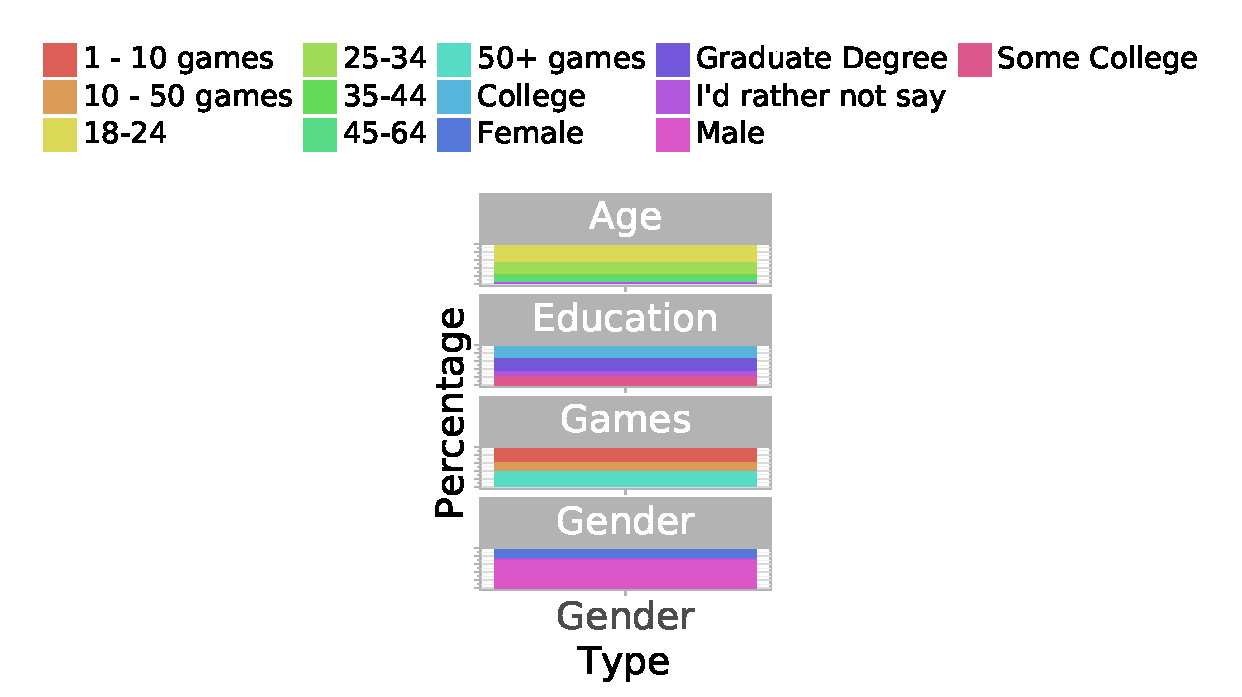
\includegraphics[width=\linewidth]{\autofig/UserDemographics.pdf}
%	\label{fig:questions1}
%	\caption{Demographics vary in these dimensions.  Not pictured are the plots showing that most users are male and speak English as a primary language.}
%	
%\end{figure}
